\documentclass{beamer}
\mode<presentation>{}

\usepackage{hyperref}
\usepackage{amsmath}
\usepackage{graphicx}
\usepackage{listings}
\usepackage{color}

\beamertemplatenavigationsymbolsempty
\setbeamertemplate{footline}[frame number]

\graphicspath{ {/Users/matthew.drury/Lectures/boosting-presentation/plots/} }

\AtBeginSection[]{
  \begin{frame}
  \vfill
  \centering
  \begin{beamercolorbox}[sep=8pt,center,shadow=true,rounded=true]{title}
    \usebeamerfont{title}\insertsectionhead\par%
  \end{beamercolorbox}
  \vfill
  \end{frame}
}

\definecolor{mygreen}{rgb}{0,0.6,0}
\definecolor{mygray}{rgb}{0.5,0.5,0.5}
\definecolor{mymauve}{rgb}{0.58,0,0.82}

% Code formatting stuff.
\lstset{ %
  backgroundcolor=\color{white},   % choose the background color; you must add \usepackage{color} or \usepackage{xcolor}
  basicstyle=\scriptsize,          % the size of the fonts that are used for the code
  breakatwhitespace=false,         % sets if automatic breaks should only happen at whitespace
  breaklines=true,                 % sets automatic line breaking
  captionpos=b,                    % sets the caption-position to bottom
  commentstyle=\color{mygreen},    % comment style
  deletekeywords={...},            % if you want to delete keywords from the given language
  escapeinside={\%*}{*)},          % if you want to add LaTeX within your code
  extendedchars=true,              % lets you use non-ASCII characters; for 8-bits encodings only, does not work with UTF-8
  keepspaces=true,                 % keeps spaces in text, useful for keeping indentation of code (possibly needs columns=flexible)
  keywordstyle=\color{blue},       % keyword style
  language=Octave,                 % the language of the code
  otherkeywords={*,...},           % if you want to add more keywords to the set
  numbers=none,                    % where to put the line-numbers; possible values are (none, left, right)
  numbersep=5pt,                   % how far the line-numbers are from the code
  numberstyle=\tiny\color{mygray}, % the style that is used for the line-numbers
  showspaces=false,                % show spaces everywhere adding particular underscores; it overrides 'showstringspaces'
  showstringspaces=false,          % underline spaces within strings only
  showtabs=false,                  % show tabs within strings adding particular underscores
  stepnumber=2,                    % the step between two line-numbers. If it's 1, each line will be numbered
  stringstyle=\color{mymauve},     % string literal style
  tabsize=2,	                   % sets default tabsize to 2 spaces
  title=\lstname                   % show the filename of files included with \lstinputlisting; also try caption instead of title
}


\DeclareMathOperator*{\argmin}{arg\,min}
\DeclareMathOperator*{\bias}{bias}
\DeclareMathOperator*{\var}{var}
\DeclareMathOperator*{\tr}{tr}
\DeclareMathOperator*{\pd}{pd}
\DeclareMathOperator*{\goesto}{\rightarrow}
%\DeclareMathOperator*{\implies}{\Rightarrow}

\title{Boosting}
\author{Matthew Drury}

\begin{document}
%
\begin{frame}
  \titlepage
\end{frame}
%
\begin{frame}
  Boosting encompasses an \textbf{entire family} highly successful learning algorithms.
\end{frame}
%
\begin{frame}
Boosting can adapt itself effortlessly to very non-linear objectives
  \only<1>{
    \begin{figure}
      \includegraphics[scale=0.50]{sin-with-data}
    \end{figure}
   }
   \only<2>{
    \begin{figure}
      \includegraphics[scale=0.50]{sin-with-data-and-booster}
    \end{figure}
   }
   \only<3>{
    \begin{figure}
      \includegraphics[scale=0.50]{broken-sin-with-booster}
    \end{figure}
   }
\end{frame}
%
\begin{frame}
Boosting accomplishes this by \textit{growing the model gradually}
  \begin{figure}
    \includegraphics[scale=0.40]{boosting-over-time-multiple-plots}
  \end{figure}
\end{frame}
%
\begin{frame}
At each stage of the growth, the next model is built as a \textbf{small adjustment} to the previous model
  \begin{figure}
    \includegraphics[scale=0.50]{boosting-over-time-single-plot}
  \end{figure}
\end{frame}
%
\begin{frame}

\only<2->{  
\textbf{Compared to}:\\~\\
}

\only<1>{
\textbf{Boosting}: \\~\\
Lowers variance by growing the model slowly over time (along with a few other tricks).\\~\\

Lowers bias by stacking many small models into the final result.
}

\only<2-3>{
\textbf{Linear Models}: \\~\\
Lowers variance by \only<3->{using a regularization penalty.}\\~\\

Lowers bias by \only<3->{including more features.}
}

\only<4-5>{
\textbf{Random Forest}: \\~\\

Lowers variance by \only<5>{growing many learners on different subsamples of the data and predictors, then averaging them.}\\~\\

Lowers bias by \only<5>{growing really big trees.}
}

\end{frame} % Introduction
\section{Outline of the Lesson}
%
\begin{frame}
\textbf{Agenda:}
 
  \begin{itemize}
    \item Introduction
    \item Boosting To The Residuals
    \item Practical Gradient Boosted Regression
    \item Interpreting Gradient Boosted Regression
    \item Boosting for Classification.
    \item Drawbacks of Boosting
    \item Software Options
  \end{itemize}

\end{frame}
%
\begin{frame}
\textbf{Objectives:}

  \begin{itemize}
    \item Understand the conceptual foundation of Boosting
    \item Understand the algorithm's hyperparameters, and how to tune them.
    \item Understand some basic strategies for interpreting a booster.
    \item Understand when boosting is appropriate, and when it is not.
    \item Be aware of the possibility of creating your own loss function.
  \end{itemize}
  
\end{frame} % Outline and Goals
\section{Boosting To Residuals}

\begin{frame}
Let's start with our usual basic setup.\\~\\

$\{ x_i, y_i \}$ is a data set, where $i$ indexes the samples we have available for training our model.\\~\\

Each $x_i$ may be a vector, in which case I'll refer to it's components (if needed) as $x_{ij}$.\\~\\

If needed, $N$ will be the number of training samples, and $M$ the number of features.
\end{frame}
%

\begin{frame}
Our goal is to construct a function $f$ so that

$$ y_i \approx f(x_i) \ \text{for all} \ i $$

\end{frame}
%

\begin{frame}
To be more precise, let's look for an $f$ so that 

$$ \sum_i \left( y_i - f(x) \right)^2 $$

is small.
\end{frame}
%

\begin{frame}
As we saw in the introduction, we would like to build up $f$ in stages, making small adjustments as we go along.

  \begin{figure}
    \includegraphics[scale=0.40]{boosting-over-time-multiple-plots}
  \end{figure}
  
\end{frame}
%

\begin{frame}
In the end, $f$ will be a sum of smaller models (often called \textit{weak learners})

$$ f(x) = f_0(x) + f_1(x) + f_2(x) + \cdots + f_{\text{max}}(x) $$

The process of building up the model looks like

\begin{align*}
    S_0(x) &= f_0(x) \\
    S_1(x) &= f_0(x) + f_1(x) \\
    S_2(x) &= f_0(x) + f_1(x) + f_2(x) \\
    &\vdots \\
    S_{\text{max}}(x) &= f_0(x) + f_1(x) + f_2(x) + \cdots + f_{\text{max}}(x) \\
\end{align*}
\end{frame} 
%

\begin{frame}{Where Should We Start?}
We want to make the simplest possible choice for our first stage

$$ f_0(x) = \text{constant} $$

But what constant?
\end{frame}
%

\begin{frame}
We are trying to minimize the sum of squared errors, so a good choice would be to find the constant minimizing

$$ \sum_i \left( y_i - \text{constant} \right)^2 $$

\textbf{Question}: What is the correct choice here?
\end{frame}
%

\begin{frame}
$$ f_0(x) = \frac{1}{N} \sum_i y_i $$
\end{frame}
%

\begin{frame}{How To Update}
We are now in the situation illustrated below

  \begin{figure}
    \includegraphics[scale=0.40]{zeroth-boosting-stage}
  \end{figure}

Our next task is to update our simple $f_0$ to $S_1(x) = f_0(x) + f_1(x)$.

\end{frame}
%

\begin{frame}
Intuitively, it's obvious what we should do

  \begin{figure}
    \includegraphics[scale=0.50]{zeroth-boosting-stage-what-to-do}
  \end{figure}
\end{frame}
%

\begin{frame}
But how can we use \textit{the data} to tell us this?  We won't always have the luxury of such simple pictures.

  \begin{figure}
    \includegraphics[scale=0.50]{zeroth-boosting-stage-what-to-do}
  \end{figure}
  
\end{frame}
%
\begin{frame}
Take a moment to think: how is the data is telling us what to do?

  \begin{figure}
    \includegraphics[scale=0.50]{zeroth-boosting-stage-what-to-do}
  \end{figure}
  
\end{frame}
%

\begin{frame}
The \textit{residuals}, $y_i - f_0(x_i)$ answer this question

  \begin{figure}
    \includegraphics[scale=0.50]{first-boosting-stage-with-residuals}
  \end{figure}
\end{frame}
%

\begin{frame}
  \begin{center}
    \textbf{We should adjust $f_0(x)$ in the direction of the residuals!}\\~\\
  \end{center}

\only<2>{
  \begin{center}
    But...  there is a big issue with this...
  \end{center}
}

  \begin{figure}
    \includegraphics[scale=0.50]{first-boosting-stage-with-residuals}
  \end{figure}
  
\end{frame}
%

\begin{frame}

  \begin{figure}
    \includegraphics[scale=0.60]{first-boosting-stage-with-residuals-dillema}
  \end{figure}
  
\end{frame}
%

\begin{frame}
We can only calculate residuals \textit{at the training data points}!

  \begin{figure}
    \includegraphics[scale=0.40]{first-boosting-stage-with-residuals-dillema}
  \end{figure}

We need some way of \textbf{extending} the values of the residuals to places we \textit{do not have data}.
\end{frame}
%

\begin{frame}
\textbf{Solution:}\\~\\

\only<2->{Fit a model to the residuals!\\~\\}

\only<3->{
  The \textbf{predictions from this model} both:
  \begin{itemize}
    \item Approximate the residuals at the places we \textit{have} data.
    \item Are defined everywhere.
  \end{itemize}
}
\end{frame}
%

\begin{frame}
Here is a \textit{new} dataset.

\begin{itemize}
  \item The values of $x$ are the same as before, taken directly from the training data.
  \item The response values are the \textit{residuals}: $y_{\text{new}} = y_i - f_0(x_i)$.
\end{itemize}

  \begin{figure}
    \includegraphics[scale=0.40]{first-boosting-stage-residual-training-set}
  \end{figure}
  
\end{frame}
%

\begin{frame}
Here is a very simple model fit to this \textit{working data set}

  \begin{figure}
    \includegraphics[scale=0.50]{first-boosting-stage-residuals-with-tree}
  \end{figure}

\end{frame}
%

\begin{frame}
Now we can update the model.

$$S_1(x) = f_0(x) + f_1(x) \leftarrow \text{Model fit to residuals!}$$

  \begin{figure}
    \includegraphics[scale=0.40]{second-boosting-stage}
  \end{figure}
  
\end{frame}
%

\begin{frame}
  \begin{center}
    Let's go one more step, so that the idea is clear.
  \end{center}
\end{frame}
%

\begin{frame}
Calculate the residuals of the current model...

  \begin{figure}
    \includegraphics[scale=0.50]{second-boosting-stage-with-residuals}
  \end{figure}
  
\end{frame}
%

\begin{frame}
Create a training data set with the residuals as the response...

  \begin{figure}
    \includegraphics[scale=0.50]{second-boosting-stage-residual-training-set}
  \end{figure}
  
\end{frame}
%

\begin{frame}
Create a training data set with the residuals as the response...

  \begin{figure}
    \includegraphics[scale=0.50]{second-boosting-stage-residuals-with-tree}
  \end{figure}
  
\end{frame}
%

\begin{frame}
Update the model!

  \begin{figure}
    \includegraphics[scale=0.50]{third-boosting-stage}
  \end{figure}
  
\end{frame}
%

\begin{frame}

  \begin{figure}
    \includegraphics[scale=0.60]{simple-boosting-over-time}
  \end{figure}
  
\end{frame}
%

\begin{frame}{But, What Happened to Growing Slowly Over Time?}
Instead of adding in the entirety of the residual fitted tree during an update

$$ S_{k+1}(x) = S_{k}(x) + f_{k+1}(x) $$

Instead we added some \textit{small fraction} of $f_{k+1}$

$$ S_{k+1}(x) = S_{k}(x) + \lambda f_{k+1}(x) $$
\end{frame}
%

%

\begin{frame}
$$ \lambda = 0.01 $$

  \begin{figure}
    \includegraphics[scale=0.50]{simple-boosting-over-time-learning-rate}
  \end{figure}

\end{frame}
%

\begin{frame}{Gradient Boosting to Minimize Sum of Squared Errors}

\textbf{Inputs:} A training data set $\{ x_i, y_i \}$, and a learning rate $\lambda$.

\textbf{Returns:} A function $f$ such that $f(x_i) \approx y_i$.

\begin{itemize}
  \item Initialize $S_0(x) = f_0(x) = \frac{1}{N} \sum_i y_i$.
  \item Iterate (parameter $k$) until satisfied: \begin{itemize}
    \item Create the working data set $W_k = \{ x_i, y_i - S_{k}(x_i) \}$.
    \item Fit a regression tree to $W_k$, minimizing least squares.  Call this tree $f_k$.
    \item Set $S_{k+1}(x) = S_{k}(x) + \lambda f_{k}(x)$. 
  \end{itemize}
  \item Return $f_{\text{max}}(x) = f_0(x) + f_1(x) + f_2(X) + \cdots + f_{\text{max}}(x)$.
\end{itemize}

\end{frame}
%

\begin{frame}{Why is it Called Gradient Boosting?}
Remember when we were in this situation:

  \begin{figure}
    \includegraphics[scale=0.35]{first-boosting-stage-with-residuals}
  \end{figure}
  
We want to use the residuals to update the model

$$ S_{k+1}(x_i) = S_{k}(x_i) + \lambda (y_i - S_{k}(x_i)) $$

\end{frame}
%

\begin{frame}
Removing the details of the specific situation, this looks like

$$ S_{k+1}(x_i) = S_{k}(x_i) + \lambda (y_i - S_{k}(x_i)) $$
$$ \Downarrow $$
$$ \xi_{k+1} = \xi_k + \lambda (y - \xi_k) $$

\textbf{Question:} Does this look... familiar?
\end{frame}
%

\begin{frame}

\only<1>{
\textbf{Recall}: Gradient descent is a general purpose algorithm for optimizing any objective function $L(x)$.\\~\\

  \begin{center}
    \textit{How does this go?}
  \end{center}
}

\only<2>{
\textbf{Algorithm:} Gradient Descent to Minimize a function $L$.\\~\\

\textbf{Inputs:} A function $L$.

\textbf{Outputs:} A point $x_{\text{optim}}$ that minimizes $L$. \\~\\

\begin{itemize}
  \item Compute $\nabla L(x)$ somehow, on paper is good.
  \item Initialize $x_0 = 0$ (arbitrary, there may be more principled choices).
  \item Iterate until convergence: \begin{itemize}
    \item Set $x_{i+1} = x_i - \lambda \nabla L(x_i)$.
  \end{itemize}
\end{itemize}
}

\end{frame}
%

\begin{frame}
What happens when we apply gradient descent to minimize the squared error loss?

$$ L(\xi, y) = \frac{1}{2} \left( y - \xi \right)^2 $$
\end{frame}
%

\begin{frame}
$$ - \nabla_{\xi} L (\xi, y) = - \frac{1}{2} \frac{\partial}{\partial \xi} \left( y - \xi \right)^2 = y - \xi $$
\end{frame}
%

\begin{frame}
So gradient descent for least squares looks like...

$$\xi_{k+1} = \xi_{k} - \lambda \nabla_{\xi} L (\xi_k, y) = \xi_{k} + \lambda (y - \xi_{k})$$

That is, \textbf{least squares gradient descent iteratively moves in the direction of the residual}.
\end{frame}
%

\begin{frame}
This is why the algorithm is called \textbf{Gradient Boosted Regression}.\\~\\

We "boost" the current estimate by adding an \textit{approximation to the gradient of the squared error loss function}.
\end{frame}

 % You Could Have Invented Gradient Boosting
\section{Practical Gradient Boosted Regression}
%
\begin{frame}[fragile]
Scikit-learn includes the gradient boosted regression algorithm in the \texttt{ensembles} module\\~\\

\begin{lstlisting}[language=python]
from sklearn.ensemble import GradientBoostedRegressor
\end{lstlisting}

\end{frame}
%
\begin{frame}[fragile]
A \texttt{GradientBoostingRegressor} object is fit in the same way as every other leaning model in sklearn\\~\\

\begin{lstlisting}[language=python]
model = GradientBoostingRegressor()
model.fit(X, y)
\end{lstlisting}

\end{frame}
%
\begin{frame}[fragile]
The \texttt{predict} method returns predictions on new data\\~\\

\begin{lstlisting}[language=python]
preds = model.predict(X_new)
\end{lstlisting}
\end{frame}
%

\begin{frame}[fragile]
Especially useful is the iterator \texttt{staged\_predict} which creates predictions from models created by truncating series of trees\\~\\

\begin{lstlisting}[language=python]
for preds in model.staged_predict(X_new):
    # Do something interesting, used heavily in the plots to follow.
\end{lstlisting}

\end{frame}
%
\begin{frame}[fragile]

\texttt{GradientBoostingRegressor} has many knobs to turn.\\~\\

\begin{lstlisting}[language=python]
GradientBoostingRegressor(loss='ls',
                          n_estimators=100, 
                          learning_rate=0.1,
                          max_depth=3,
                          subsample=1.0, 
                          min_samples_split=2, 
                          min_samples_leaf=1, 
                          min_weight_fraction_leaf=0.0,
                          ...)
\end{lstlisting}

\end{frame}
%
\begin{frame}[fragile]
The most important options to \texttt{GradientBoostedRegressor} are

\begin{itemize}
  \item \texttt{loss} controls the loss function to minimize.  \texttt{ls} is the least squares minimization algorithm we discussed in the previous section.
  \item \texttt{n\_estimators} is how many boosting stages to compute, i.e. how many regression trees to grow.
  \item \texttt{learning\_rate} is the learning rate for the gradient update.
  \item \texttt{max\_depth} controls how deep to grow each individual tree.
  \item \texttt{subsample} allows to fit each tree on a random sample of the training data (similar to bagging in random forests).
\end{itemize}

\end{frame}
%
\begin{frame}{Tuning the Number of Estimators}

As more and more trees are added to the model the training set error will be driven down monotonically, but the same is not true for the testing error

  \begin{figure}
    \includegraphics[scale=0.45]{training-and-testing-error}
  \end{figure}

\end{frame}
%
\begin{frame}{Tuning the Number of Estimators}

\textbf{Question:} Will the training error ever become \textit{exactly} zero?

  \begin{figure}
    \includegraphics[scale=0.45]{training-and-testing-error}
  \end{figure}

\end{frame}
%
\begin{frame}

  \begin{figure}
    \includegraphics[scale=0.45]{training-and-testing-error}
  \end{figure}

This means that it is essential to determine the proper number of trees to grow, as too many may lead to overfitting

\end{frame}
%
\begin{frame}
One way to tune the number of trees is to make use of a validation set, held out from training the model

  \begin{figure}
    \includegraphics[scale=0.45]{training-and-testing-error-with-optima}
  \end{figure}
  
\end{frame}
%
\begin{frame}[fragile]
The \texttt{loss\_} method is important here, it allows us to compute the loss function on held out data\\~\\

\begin{lstlisting}[language=python]
def get_optimal_n_estimators(model, X_new, y_new):
    validation_loss = np.zeros(
        model.get_params('n_estimators'))
    for i, preds in enumerate(model.staged_predict(X_new)):
        validation_loss[i] = model.loss_(preds, y_new)    
    optimal_tree = np.argmin(validation_loss)
    optimal_loss = validation_loss[optimal_tree]
    return optimal_tree, optimal_loss
\end{lstlisting}

\end{frame}
%
\begin{frame}[fragile]
One the optimal number of estimators is known, it's useful to truncate the model\\~\\

\begin{lstlisting}[language=python]
from copy import deepcopy

def truncate_boosted_model(model, n_estimators):
    new_model = deepcopy(model)
    # Two dimensions here for the case of multiple classes
    # in a GradientBoostedClassifier.
    new_model.estimators_ = model.estimators_[:n_estimators, :]
    new_model.n_estimators = n_estimators
    return new_model
\end{lstlisting}

\end{frame}
%
\begin{frame}
Another way to choose the optimal number of trees is to replace the validation set with cross validation

  \begin{figure}
    \includegraphics[scale=0.45]{training-and-testing-cv-error}
  \end{figure}
  
\end{frame}
%
\begin{frame}

  \begin{figure}
    \includegraphics[scale=0.45]{training-and-testing-cv-error}
  \end{figure}
  
We generally choose the number of trees minimizing the \textit{average} out validation fold error.

\end{frame}
%
\begin{frame}{Tuning the Learning Rate}

The learning rate allows us to grow our boosted model slowly.\\~\\

A large learning rate will cause the model to fit hard to the training data, which creates a \textit{high variance} situation.\\~\\

A smaller learning rate reduces the boosted models sensitivity to the training data.\\~\\

\end{frame}
%
\begin{frame}
Decreasing the learning rate reduces how fast the booster drives down the training error rate
  \begin{figure}
    \includegraphics[scale=0.50]{varying-learning-rate-error-training}
  \end{figure}
  
\end{frame}
%
\begin{frame}
On the other hand, a smaller learning rate means more trees are needed to reach the optimal point

  \begin{figure}
    \includegraphics[scale=0.50]{varying-learning-rate-error-testing-zoom-start}
  \end{figure}
  
\end{frame}
%
\begin{frame}
In general, a smaller learning rate eventually (over enough time) results in a superior model

  \begin{figure}
    \includegraphics[scale=0.50]{varying-learning-rate-error-testing-zoom-end}
  \end{figure}
  
\end{frame}
%
\begin{frame}
\textbf{Strategy for Tuning Learning Rate}:

\begin{itemize}
  \item In the initial exploratory phases of modeling, set the learning rate to some large value, say $0.1$.  This allows you to iterate through ideas quickly.
  \item When tuning other parameters using grid search, decrease the learning rate to a more sensible value, $0.01$ works well.
  \item When fitting the \textit{final} production model, set the learning rate to a very small value, $0.001$ or $0.0005$, smaller is better.
\end{itemize}

\end{frame}
%
\begin{frame}
\textbf{General Advice:}\\~\\

Run the final model overnight!  It will fit while you are sleeping!\\~\\

Make sure you've written all your analysis code up front, based on your initial models.  Then all that's left is to run your final model through and see your final plots and statistics.
\end{frame}

%
\begin{frame}{Tuning the Tree Depth}
A larger tree depth allows the model to capture deeper interactions between the predictors, resulting in lower bias.

  \begin{figure}
    \includegraphics[scale=0.3]{sin-changing-depth}
  \end{figure}

\end{frame}
%
\begin{frame}
A deeper tree depth also

\begin{itemize}
  \item Causes the model to fit faster, increasing the variance and somewhat combating the effect of the learning rate.
  \item Allows the model to assume a more complex for at the same number of trees.  This is a blessing (low bias) and curse (high variance).
\end{itemize}
\end{frame}
%
\begin{frame}
It's never obvious up front what tree depth is best for a given problem, so a grid search is needed to determine the best value

  \begin{figure}
    \includegraphics[scale=0.50]{varying-tree-depth-error}
  \end{figure}
  
\end{frame}
%
\begin{frame}

  \begin{figure}
    \includegraphics[scale=0.50]{varying-tree-depth-error-zoom}
  \end{figure}
  
\end{frame}
%
\begin{frame}
\textbf{Strategy for Tuning Tree Depth}:

Tune with a grid search and cross validation.
  
\end{frame}
%
\begin{frame}{Tuning the Subsample Rate}
The \texttt{subsample} parameter allows one to train each tree on a subsample of the training data.\\~\\

This is similar to bagging in the random forest algorithm, and has the same result: it lowers the variance of the resulting model.
\end{frame}
%
\begin{frame}
Not subsampling at all, or over subsampling are both bad ideas

  \begin{figure}
    \includegraphics[scale=0.50]{varying-subsample-rate-error}
  \end{figure}
 
\end{frame}
%
\begin{frame}
Between these two extremes, different levels of subsampling generally give the same performance

  \begin{figure}
    \includegraphics[scale=0.50]{varying-subsample-rate-error-zoom-end}
  \end{figure}
  
\end{frame}
%


\begin{frame}
\textbf{Question}: Why does the training error sometimes \textit{increase} when the learning rate is $1.0$?

  \begin{figure}
    \includegraphics[scale=0.50]{varying-learning-rate-error-training}
  \end{figure}
  
\end{frame}
%

\begin{frame}
\textbf{Strategy For Tuning Subsample:}\\~\\

Set to $0.5$, it almost always works well.\\~\\

If you have a massive amount of data and want the model to fit more quickly, decrease this value.\\~\\

\textbf{Note:} The default rate in sklearn is $1.0$, so make sure you \textit{always} change it.
\end{frame}
%
\begin{frame}{Tuning Other Gradient Boosting Parameters}

The other parameters to \texttt{GradientBoostingRegressor} are less important, but can be tuned with grid search for additional improvements in importance.

\begin{itemize}
  \item \texttt{min\_samples\_split}: Any node with less samples than this will not be considered for splitting.
  \item \texttt{min\_samples\_leaf}: All terminal nodes must contain more samples than this.
  \item \texttt{min\_weight\_fraction\_leaf}: Same as above, but a expressed as a fraction of the total number of training samples.
\end{itemize}

\end{frame}
%
\begin{frame}
Generally these are less important because \textit{you shouldn't be growing super gigantic trees}!\\~\\
\end{frame}

\begin{frame}

\textbf{Question:} Is there any risk to including these parameters in a grid search and selecting the best using cross validation?\\~\\

\only<2->{
If you \textit{do} decide to include these in a grid search, \textit{be wary of overfitting to your validation set}.\\~\\
}

\only<3->{
\textit{The number of model comparisons grows exponentially in the number of parameters tuned.}
}
\end{frame}
%
\begin{frame}{Max Features}
There's one more parameter worth mentioning\\~\\

\texttt{max\_features}: The number of features to consider for each split, as in random forest.\\~\\

\textbf{Exercise}: Think about how varying this parameter will influence the model.  Run some experiments to see if you're right.  Should you include this in a grid search?
\end{frame}
  
  
 % Practical Gradient Boosted Regression
\section{Interpreting Gradient Boosting}

\begin{frame}
Gradient boosting models, while offering massive predictive power, are very complex and hard to interpret.
\end{frame}
%
\begin{frame}
There are two high level summarization techniques that are very popular, and can help understand the high level content of the model and diagnose issues

\begin{itemize}
  \item \textbf{Relative Variable Importance}: Measures the amount a predictor "participates" in the model fitting procedure.
  \item \textbf{Partial Dependence Plots}: Are analogous to parameter estimates in linear regressions, they summarize the effect of a single predictor while controlling for the effect of all others.
\end{itemize}
\end{frame}
%
\begin{frame}{Relative Variable Importance}
The concept here is the same as in random forest.\\~\\

\only<2->{
Each time we grow a tree, we keep track of how much the error metric decreases at each split, and allocate that decrease to a predictor.\\~\\
}

\only<3->{
The importance of a predictor \texttt{in a tree} is the total amount the error metric decreased over all splits on that predictor\\~\\
}

\only<4->{
The importance of a predictor in the boosted model is the \texttt{average} importance of the predictor over all the trees.
}

\end{frame}
%
\begin{frame}
It is traditional to normalize the importances so that they sum to $100$.

  \begin{figure}
    \includegraphics[scale=0.45]{feature-importances}
  \end{figure}
  
\end{frame}
%
\begin{frame}
\textbf{Comments:}\\~\\

\begin{itemize}

\only<1>{
    \item The name "feature importances" is pretty awful.  It invites misinterpretation.  
    \begin{center}
    \textit{Don't reason about things from the names they have been given, make sure the statistic actually answers your question}.
    \end{center}
}

\only<2>{
    \item If your model contains both numeric and binary predictors, the importance metric is biased to assign higher values to the numeric predictors.  Try not to compare feature importances across these two classes.
}

\only<3>{
    \item Feature importance rankings can have very high variance.  Make sure
    any important conclusions are robust to different RNG seeds and training sets.
}

\only<4>{
    \item Make sure your model only includes trees \textit{up to the optimal point}.  Otherwise you'll allocate importance to overfitting.
}

\only<5>{
    \item Dominant features should be treated with suspicion.  They can often be a sign of data leakage.
}
\end{itemize}
\end{frame}
%

\begin{frame}{Partial Dependence Plots}

Visualizations of the effect of a single predictor, averaging out the effects of all the rest

  \begin{figure}
    \includegraphics[scale=0.33]{patial-dependence-plots}
  \end{figure}

\end{frame}
%
\begin{frame}
In symbols:

$$ \pd_j(x) = \frac{1}{N} \sum_i f(\overbrace{x_{i1}, x_{i2}}^{\text{The training data points}}, \ldots, \overbrace{x}^{\text{The j'th spot}}, \ldots, x_{iM}) $$
\end{frame}
%
\begin{frame}
By varying the values of two predictors, we can draw partial dependence plots in higher dimensions

  \begin{figure}
    \includegraphics[scale=0.45]{patial-dependence-plot-two-features}
  \end{figure}
 
\end{frame}
%
\begin{frame}
\textbf{Question:} Does it look like any trees split on \textit{both} RM and DIS?

  \begin{figure}
    \includegraphics[scale=0.45]{patial-dependence-plot-two-features}
  \end{figure}
 
\end{frame}
%
\begin{frame}
\textbf{Question:} What about AGE and DIS?

  \begin{figure}
    \includegraphics[scale=0.45]{patial-dependence-plot-two-features-with-interaction}
  \end{figure}
 
\end{frame}
 % Partial Dependence Plots + Variable Importance
\section{Other Gradient Boosting Algorithms}

\begin{frame}
The last great feature of Gradient Boosting is that it generalizes easily to other loss functions.
\end{frame}
%
\begin{frame}
We will discuss two generalizations:

\begin{itemize}
  \item \textbf{Gradient Boosted Logistic Regression}: Minimizes the binomial deviance (logistic log likelihood) loss function.
  \item \textbf{AdaBoost}: Minimizes a custom classification loss.
\end{itemize}

It is important to say: \textit{There are many more possibilities}!
\end{frame}
%
\begin{frame}{Gradient Boosted Logistic Regression}
We want to generalize our boosting algorithm to also solve \textit{classification} problems. 

$$ y \in  \{0, 1\} $$

We want to estimate $ f(x) = Pr(y = 1 \mid x) $.
\end{frame}
%
\begin{frame}
For example, here is a complex classification problem

  \begin{figure}
    \includegraphics[scale=0.45]{classification-boundary-with-data}
  \end{figure}

\end{frame}
%
\begin{frame}
How would you solve this with standard logistic regression?

  \begin{figure}
    \includegraphics[scale=0.45]{classification-boundary-with-data}
  \end{figure}

\end{frame}
%
\begin{frame}
Gradient boosted logistic regression makes short work of it.

  \begin{figure}
    \includegraphics[scale=0.45]{classification-boundary-with-booster}
  \end{figure}

\end{frame}
%
\begin{frame}
Recall our friend \textbf{logistic regression}.

$$ \hat \beta = \argmin_{\beta} \sum_i \left( y_i \nu(\beta, x_i) - \log(1 + e^{\nu(\beta, x_i)}) \right) $$

Where $\nu(\beta, x_i) = \beta_0 + \beta_1 x_{i1} + \cdots + \beta_{M} x_{iM}$.\\~\\ 

The quantity $\nu$ is called the \textit{linear predictor}.\\~\\

In logistic regression it represents the \textit{log odds} of the outcome.
\end{frame}
%
\begin{frame}
Once we have solved for $\hat \beta$, we can make predictions using

$$p(x) = \frac{1}{1 + e^{-(\hat \beta_0 + \hat \beta_1 x_1 + \cdots + \hat \beta_M x_M)}}$$

The predictions can interpreted as \textit{the conditional probability that $y = 1$, given the values of $x$}.

$$ p(x) = Pr(y = 1 \mid x) $$
\end{frame}
%
\begin{frame}
The function we are minimizing in logistic regression is called the \textit{logistic loss}:

$$ L(f, y) = y f - \log(1 + e^{f}) $$

  \begin{figure}
    \includegraphics[scale=0.42]{loss-function-logistic}
  \end{figure}
  
\end{frame}
%
\begin{frame}
  \begin{center}
    \textbf{Logistic regression can be solved with gradient descent.}
  \end{center}
\end{frame}
%
\begin{frame}
\textbf{Gradient Boosted Logistic Regression}:\\~\\
Replace the linear predictor in logistic regression 

$$\nu(\beta, x) = \beta_0 + \beta_1 x_1 + \cdots + \beta_{M} x_M$$

With a sum of small regression trees

$$\nu(x) = T_0(x) + T_1(x) + \cdots + T_{\text{max}}(x)$$
\end{frame}
%
\begin{frame}
To fit a Gradient Boosted Logistic Regression, replace the least squares loss function

$$ L(f, y) = \frac{1}{2} \left(f - y \right)^2 $$

With the logistic loss

$$ L(f, y) = y f - \log(1 + e^f) $$

And then use the same gradient boosting technique.

\end{frame}
%
\begin{frame}
The gradient of the logistic loss is

\begin{align*}
\nabla_f L(f, y) &= \frac{\partial}{\partial f} \left( y f - \log(1 + e^f) \right) \\
&= y - \frac{e^f}{1 + e^f} \\
&= y - p(f)
\end{align*}

So we can interpret this method as "boosting to the residual probabilities".
\end{frame}
%

\begin{frame}
\textbf{Note:} There are some subtleties.  I'll include some extra readings in the weekend email.
\end{frame}
%
\begin{frame}[fragile]
Gradient boosted logistic regression is implemented in sklearn as\\~\\

\begin{lstlisting}[language=python]
from sklearn.ensembles import GradientBoostingClassifier
model = GradientBoostingClassifier()
# Now y must be a np.array of 0 and 1's!
model.fit(X, y)
\end{lstlisting}
\end{frame}
%
\begin{frame}[fragile]
The options to \texttt{GradientBoostingClassifier} are the same as those to \texttt{GradientBoostingRegressor}\\~\\

\begin{lstlisting}[language=python]
GradientBoostingClassifier(loss='deviance',
                           n_estimators=100, 
                           learning_rate=0.1, 
                           max_depth=3,
                           subsample=1.0, 
                           min_samples_split=2, 
                           min_samples_leaf=1, 
                           min_weight_fraction_leaf=0.0,
                           ...)
\end{lstlisting}

And everything we said before generalizes.
\end{frame}
%
\begin{frame}[fragile]
To make predictions use \texttt{predict\_proba}\\~\\

\begin{lstlisting}[language=python]
model.predict_proba(X)
\end{lstlisting}

The \texttt{predict} method returns \textit{class labels} (by comparing the probability to $0.5$), making it much less useful.
\end{frame}
%
\begin{frame}[fragile]{Gradient Boosted AdaBoost}
By using the \texttt{'exponential'} loss, we get the Adaboost algorithm:

\begin{lstlisting}[language=python]
model = GradientBoostingClassifier(loss='exponential')
model.fit(X, y)
\end{lstlisting}

\end{frame}
%
\begin{frame}
The Adaboost algorithm uses labels $y \in \{-1, 1\}$ and minimizes the loss function

$$ L(f, y) = \exp( - y f) $$

  \begin{figure}
    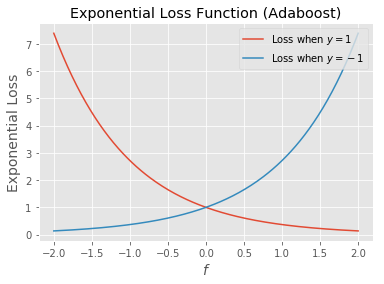
\includegraphics[scale=0.42]{loss-function-adaboost}
  \end{figure}

\end{frame}
%
\begin{frame}
The performance of Adaboost is generally comparable to that of gradient boosted logistic regression

  \begin{figure}
  
    \includegraphics[scale=0.45]{classification-boundary-with-ada-gradient-booster}
  \end{figure}
  
\end{frame}
%
\begin{frame}
In fact, the classification boundaries are \textit{the same}

  \begin{columns}
    \column{.5\textwidth}
    \begin{figure}
      \includegraphics[scale=0.28]{classification-boundary-with-booster}
    \end{figure}
    \column{.5\textwidth}
    \begin{figure}
      \includegraphics[scale=0.28]{classification-boundary-with-ada-gradient-booster}
    \end{figure}
  \end{columns}
  
\end{frame}
%
\begin{frame}
Gradient boosted logistic regression is less sensitive to outliers than Adaboost.  Can you see why?

  \begin{figure}
    \includegraphics[scale=0.45]{loss-function-comparison}
  \end{figure}
  
\end{frame}
%
\begin{frame}[fragile]
The implementation of Adaboost as a gradient booster is a somewhat recent development.\\~\\

Originally (before the invention of gradient boosting), Adaboost was accomplished by a complicated sample re-weighing scheme.\\~\\
\end{frame}
%
\begin{frame}[fragile]
The traditional Adaboost is included in sklearn as \texttt{AdaBoostClassifier}\\~\\

\begin{lstlisting}[language=python]
model = AdaBoostClassifier()
model.fit(X, y)
\end{lstlisting}

Traditional Adaboost always uses trees of depth $1$ (often playfully called "stumps", so there is no \texttt{max\_depth} argument.
\end{frame}

%
\begin{frame}[fragile]
Traditional Adaboost is outclassed by gradient boosting, but retains historical and mathematical significance

  \begin{figure}
    \includegraphics[scale=0.45]{classification-boundary-with-ada-booster}
  \end{figure}
 
\end{frame}
%
\begin{frame}{A Final Comparison of Classification Algorithms}

  \begin{figure}
    \includegraphics[scale=0.5]{classification-mixed}
  \end{figure}

\end{frame}
%
\begin{frame}

  \begin{figure}
    \includegraphics[scale=0.5]{classification-mixed-logistic-boosting}
  \end{figure}
  
\end{frame}
%
\begin{frame}

  \begin{figure}
    \includegraphics[scale=0.5]{classification-mixed-ada-gradient-boosting}
  \end{figure}
  
\end{frame}
%
\begin{frame}

  \begin{figure}
    \includegraphics[scale=0.5]{classification-mixed-ada-traditional-boosting}
  \end{figure}
  
\end{frame}
%
\begin{frame}

  \begin{figure}
    \includegraphics[scale=0.5]{classification-mixed-svm}
  \end{figure}
  
\end{frame}
%
\begin{frame}

  \begin{figure}
    \includegraphics[scale=0.5]{classification-mixed-random-forest}
  \end{figure}
  
\end{frame}
 % Other Boosting Algorithms
\section{Final Words About Boosting}

\begin{frame}
Gradient Boosting is the best off-the-shelf learning algorithm available today.\\~\\
It effortlessly produces accurate models.\\~\\
\end{frame}
%
\begin{frame}
Nonetheless, it has drawbacks.
\end{frame}
%
\begin{frame}{Drawbacks of Gradient Boosting}
\begin{itemize}

\only<1>{
  \item Boosting creates very complex models.  It can be difficult to extract intuitive, conceptual, or inferential information from them.
}

\only<2>{
  \item Boosting is difficult to explain (maybe you just learned this through experience).  It can be hard to convince business leader to accept such a black box model.
}

\only<3>{
  \item Boosted models can be difficult to implement in production environments due to their complexity.
}

\only<4>{
  \item The sequential nature of the standard boosting algorithm makes it very difficult to parallelize (compared to, for example, random forest).  Recently, there has been great progress (xgboost).
}
\end{itemize}
\end{frame}
%

\begin{frame}{Software Options For Boosting}

\begin{itemize}
  \item There are many quality open source implementations of gradient boosting algorithms:
  \begin{itemize}
    \item Sklearn, obviously :)
    \item R's \texttt{gbm} is great.  It offers many different loss functions
    and is feature rich.
    \item \texttt{xgboost} is a modern interpretation of gradient boosting, with
    many algorithmic innovations that make it faster and more accurate.  State of the art, with python interface.
    \item \texttt{H2O} offers a distributed gradient booster that can handle
    massive data sets.  Also offers a python interface.
  \end{itemize}
\end{itemize}

\end{frame}
%
\begin{frame}{Q\&A}
  \begin{itemize}
    \item Understand the conceptual foundation of Boosting
    \item Understand the algorithm's hyperparameters, and how to tune them.
    \item Understand some basic strategies for interpreting a booster.
    \item Understand the drawbacks of boosting.
    \item Be aware of the possibility of creating your own loss function.
  \end{itemize}
\end{frame}

%\include{appendix_gb_details}
\end{document}
